\documentclass{paper}

%\usepackage{times}
\usepackage{epsfig}
\usepackage{graphicx}
\usepackage{amsmath}
\usepackage{amssymb}
\usepackage{color}
\usepackage{caption}
\usepackage{subcaption}


% load package with ``framed'' and ``numbered'' option.
%\usepackage[framed,numbered,autolinebreaks,useliterate]{mcode}

% something NOT relevant to the usage of the package.
\setlength{\parindent}{0pt}
\setlength{\parskip}{18pt}
\graphicspath{{images/}}


\usepackage[latin1]{inputenc} 
\usepackage[T1]{fontenc} 


\usepackage{listings} 
\lstset{% 
   language=Matlab, 
   basicstyle=\small\ttfamily, 
} 



\title{Assignment 2}



\author{Jenni Simon\\09-116-005}
% //////////////////////////////////////////////////


\begin{document}



\maketitle


% Add figures:
%\begin{figure}[t]
%%\begin{center}
%\quad\quad   \includegraphics[width=1\linewidth]{ass2}
%%\end{center}
%
%\label{fig:performance}
%\end{figure}



\paragraph{Exercise 1}

Figure \ref{fig:EduWage} shows a plot of the dependent variable "Wage" against the independent variable "Education" (in years). We can observe a roughly linear relationship between the variables (depicted with a red line). Note that outliers have been removed from the data in a pre-processing step, as suggested in Exercise 1.
\begin{figure}[h]
\begin{center}
\quad\quad   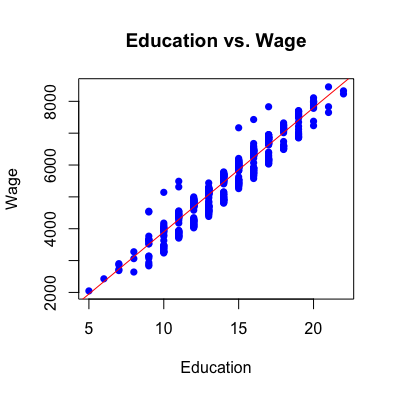
\includegraphics[width=.7\linewidth]{EduWage}
\end{center}
\caption{Plot showing years of education vs. wage. Possible relationship is depicted with a red line.}
\label{fig:EduWage}
\end{figure}


\paragraph{Exercise 2}

Figure \ref{fig:EduWageFM} shows the same data with additional color indication of gender. We can clearly observe how men (blue) tend to have a higher wage at the same amount of education. Again we observe a linear dependency between wage and education for both classes "men" and "women". 

\begin{figure}[h]
\begin{center}
\quad\quad   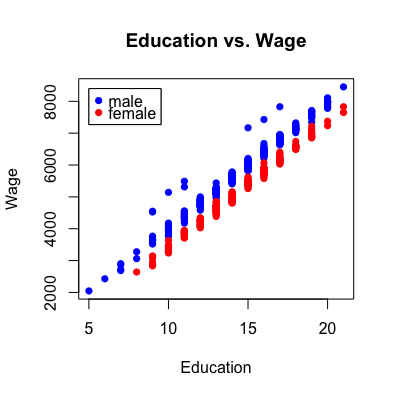
\includegraphics[width=.7\linewidth]{EduWageMF}
\end{center}
\caption{Plot showing years of education vs. wage for men (blue) and women (red).}
\label{fig:EduWageFM}
\end{figure}


\paragraph{Exercise 3}

Table \ref{tab:summary} shows the minimum, mean, median, maximum, 1st- and 2nd quantile as well as the standard deviation of the dataset after preprocessing.
The supplied dataset contained a negative time-value and  a NaN which have both been removed before the computation. Fixing the wrong sign would arguably have also been a sensible solution, as the value seems to agree with the other observations.

\begin{table}[h]
\centering
\caption{Summary of the dataset Mean20}
\label{tab:summary}
\begin{tabular}{|l|l|l|l|l|l|l|}
\hline
Min.  & 1st Qu. & Median & Mean  & 3rd Qu. & Max.  & Std.  \\ \hline 
6.850 & 6.968   & 7.010  & 7.008 & 7.072   & 7.120 & 0.075 \\ \hline
\end{tabular}
\end{table}

\paragraph{Exercise 4}
We can test the hypothesis $H_0: \mu = 7.05$ against $H_1: \mu \neq 7.05$ using Student's two-sided t-test. As the dataset is rather small, we choose a significance-level of $\alpha=0.05$. Table \ref{tab:t2proc} shows the results of this test. We observe a very low p-value (smaller than $\alpha$) and therefore reject $H_0$ in favour of $H_1$. 

\begin{table}[h]
\centering
\caption{Result of two-sided t-test on pre-processed data.}
\label{tab:t2proc}
\begin{tabular}{|c|c|c|c|}
\hline
t-value & 95\% confidence interval & p-value & Conclusion \\ \hline
-2.499 & {[}6.973, 7.043{]} & 0.0218 & $H_1$      \\ \hline
\end{tabular}
\end{table}

If we repeat the test on the original, not pre-processed data we obtain the results shown in table \ref{tab:t2orig}. We observe that the outliers have a large impact on the test results. Based on the relatively large p-value, we would accept $H_0$ in this case. 

\begin{table}[h]
\centering
\caption{Result of two-sided t-test on original data.}
\label{tab:t2orig}
\begin{tabular}{|c|c|c|c|}
\hline
t-value & 95\% confidence interval & p-value & Conclusion \\ \hline
-1.063 & {[}4.948, 7.733{]} & 0.3006 & $H_0$      \\ \hline
\end{tabular}
\end{table}

\paragraph{Exercise 5}
In this case we test the hypothesis $H_0: \mu = 7.05$ against $H_1: \mu > 7.05$ using the one-sided version of Student's t-test. The results of this test are shown in table \ref{tab:t1}. In this case we would clearly accept $H_0$. However, I would highly doubt Mary's claim with such a result (especially the extremely high p-value). 

\begin{table}[h]
\centering
\caption{Result of one-sided t-test on pre-processed data.}
\label{tab:t1}
\begin{tabular}{|c|c|c|c|}
\hline
t-value & 95\% confidence interval & p-value & Conclusion \\ \hline
-1.063 & {[}6.979, $+\infty${]} & 0.9891 & $H_0$      \\ \hline
\end{tabular}
\end{table}


 \end{document}